\section{شعر‌ فارسی}
\begin{frame}{نوشتن شعر فارسی}
\begin{itemize}\itemr
\item[-]
نوشتن شعر فارسی هم به راحتی نوشتن دیگر امکانات لاتک است.

\item[-]
برای نوشتن شعر فارسی باید از محیط 
\lr{\texttt{traditionalpoem}}
استفاده کرد.
\end{itemize}
\end{frame}

\begin{frame}[fragile]{نمونه کد}
\begin{center}
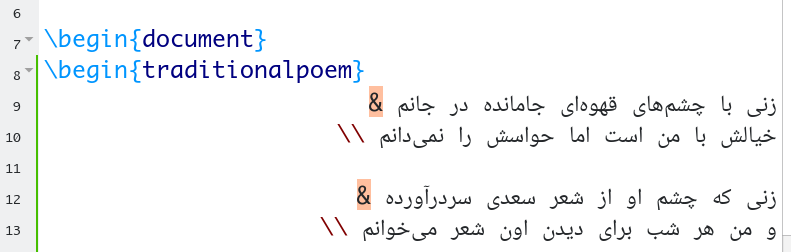
\includegraphics[width=\textwidth]{docs/images/tradpoem-code}
\end{center}
\end{frame}

\begin{frame}{خروجی}
\begin{center}
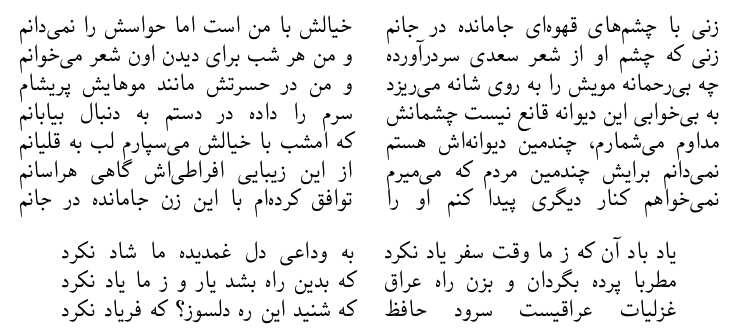
\includegraphics[width=\textwidth]{docs/images/tp-2}
\end{center}
\end{frame}
